% Fig. 2: content-driven layout, not a grid of equally weighted cards.
% The interactive path is the visual spine. Brief is an unboxed note;
% recording is a short artifact strip. Publication and measurement share
% a bottom edge, but use different widths and different internal layouts.
% Coordinates are centimetres. Every label remains horizontal.
% This is the TikZ layout before the final manual adjustments in Inkscape.
% architecture.svg is now authoritative; export it to architecture.pdf.
% Do not compile this file over the published PDF. See paper/README.md.
\documentclass[tikz,border=2pt]{standalone}
\usepackage{times}
\usepackage[T1]{fontenc}
\usepackage{textcomp}
\usepackage{graphicx}
\usetikzlibrary{arrows.meta,calc}

\definecolor{ink}{HTML}{24313D}
\definecolor{soft}{HTML}{586675}
\definecolor{rule}{HTML}{CDD5DE}
\definecolor{paperwash}{HTML}{F6F8FA}
\definecolor{blue}{HTML}{28659A}
\definecolor{bluerule}{HTML}{BDD2E4}
\definecolor{bluewash}{HTML}{EDF4FA}

\begin{document}
\begin{tikzpicture}[
  font=\sffamily\fontsize{7.5}{9.3}\selectfont,
  >={Stealth[length=1.8mm,width=1.3mm]},
  card/.style={draw=rule,fill=white,line width=0.5pt,
    rounded corners=2pt,inner sep=0,outer sep=0,anchor=north west},
  title/.style={font=\sffamily\fontsize{9}{10.5}\selectfont\bfseries,
    text=ink,inner sep=0,outer sep=0,anchor=north west,
    text height=7pt,text depth=1.6pt},
  subtitle/.style={title,font=\sffamily\fontsize{8}{9.5}\selectfont\bfseries,
    text height=6.2pt,text depth=1.5pt},
  body/.style={text=ink,inner sep=0,outer sep=0,anchor=north west,align=left},
  small/.style={body,font=\sffamily\fontsize{7.2}{8.8}\selectfont},
  note/.style={small,text=soft},
  shot/.style={inner sep=0,outer sep=0,anchor=north west},
  flow/.style={->,ink!85!white,line width=0.55pt},
  meas/.style={->,blue,line width=0.65pt},
  lab/.style={font=\sffamily\fontsize{7}{8.3}\selectfont,
    text=soft,inner sep=1.1pt,outer sep=0,align=center},
  mlab/.style={lab,text=blue},
  vlab/.style={lab,anchor=west,align=left,inner sep=0},
]

% One session encloses the worker and machine, without moving either.
\draw[draw=rule,fill=paperwash,line width=0.5pt,rounded corners=3pt]
  (3.98,0.60) rectangle (14.22,-2.46);
\node[note] at (4.2,0.40)
  {\textbf{One session}\quad one process, one private copy of the game};

% ---- Interactive spine: sizes follow the amount and type of information.
\node[card,minimum width=3cm,minimum height=1.9cm] (agent) at (0,0) {};
\node[title] at ($(agent.north west)+(0.22,-0.17)$) {Frontier model};
\node[body] at ($(agent.north west)+(0.22,-0.63)$)
  {Vision LLM in pi;\\calls the control API\\from its shell tool.};

\node[card,minimum width=3.55cm,minimum height=2.3cm] (worker) at (4.2,0) {};
\node[title] at ($(worker.north west)+(0.22,-0.17)$) {Session worker};
\node[body] at ($(worker.north west)+(0.22,-0.63)$)
  {API: screen, key\\Hold keys for emulated\\frames, then wait for\\the screen to settle.};

\node[card,minimum width=5cm,minimum height=2.3cm] (machine) at (9,0) {};
\node[title] at ($(machine.north west)+(0.25,-0.17)$) {Emulated machine};
\node[body] at ($(machine.north west)+(0.25,-0.68)$)
  {DOSBox Pure\\1996 game\\320\texttimes200 at 70 fps};
\node[shot] (mapshot) at ($(machine.north west)+(2.65,-0.65)$)
  {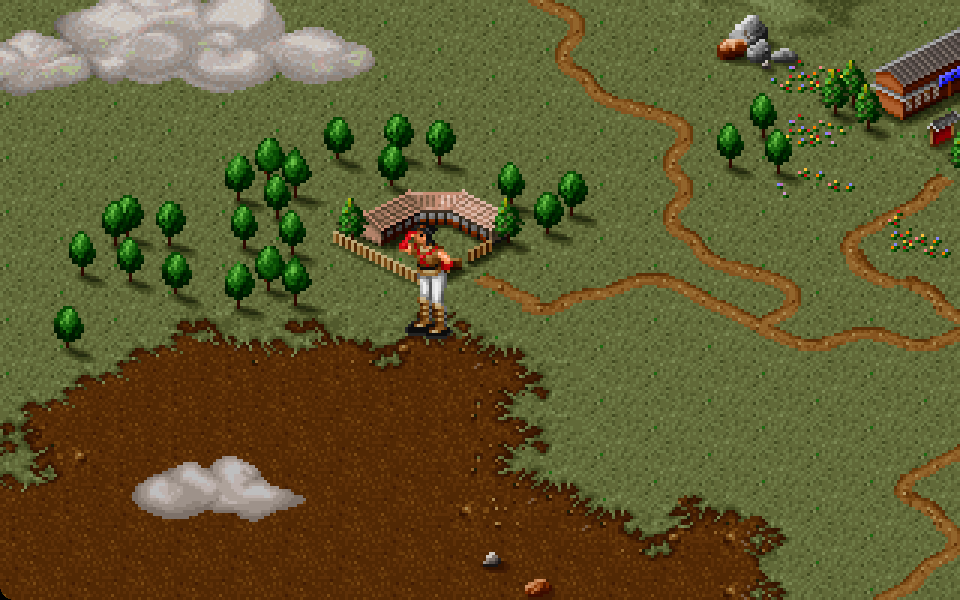
\includegraphics[width=2.1cm]{map-x3.png}};

\draw[flow] (3,-0.50) -- node[lab,above=1pt] {keys} (4.2,-0.50);
\draw[flow] (4.2,-1.10) -- node[lab,below=1pt] {frames} (3,-1.10);
\draw[flow] (7.75,-0.50) -- node[lab,above=1pt] {input} (9,-0.50);
\draw[flow] (9,-1.10) -- node[lab,below=1pt] {frames} (7.75,-1.10);

% ---- Brief: supporting input, shown as an annotation instead of a card.
\draw[rule,line width=1.2pt] (0.04,-2.65) -- (0.04,-4.05);
\node[subtitle] at (0.24,-2.70) {Brief\quad\texttt{agents.md}};
\node[note] at (0.24,-3.15)
  {Session and play calls;\\compass route; game manual.\\English and Chinese.};
\draw[flow] (1.5,-2.60) -- (agent.south);
\node[vlab] at ($(agent.south)!0.5!(1.5,-2.60)+(0.15,0)$) {read at launch};

% ---- Recording: a compact artifact strip, directly under the worker.
\node[card,fill=paperwash,minimum width=3.55cm,minimum height=1.3cm]
  (journal) at (4.2,-3.17) {};
\node[subtitle] at ($(journal.north west)+(0.22,-0.15)$) {Recording};
\node[small] at ($(journal.north west)+(0.22,-0.56)$)
  {Changed screen tiles;\\all keys and hold durations.};
\draw[flow] (worker.south) -- (journal.north);
\node[vlab] at (6.13,-2.845) {events};

% ---- Publication: two separate outputs, linked across a clear gutter.
% Both cards keep the same title, image, and bottom alignments.
\node[card,fill=paperwash,minimum width=3.2cm,minimum height=2.22cm]
  (leaderboard) at (0,-4.90) {};
\node[title] at ($(leaderboard.north west)+(0.25,-0.18)$) {Leaderboard};
\node[shot] (boardshot) at ($(leaderboard.north west)+(0.25,-0.65)$)
  {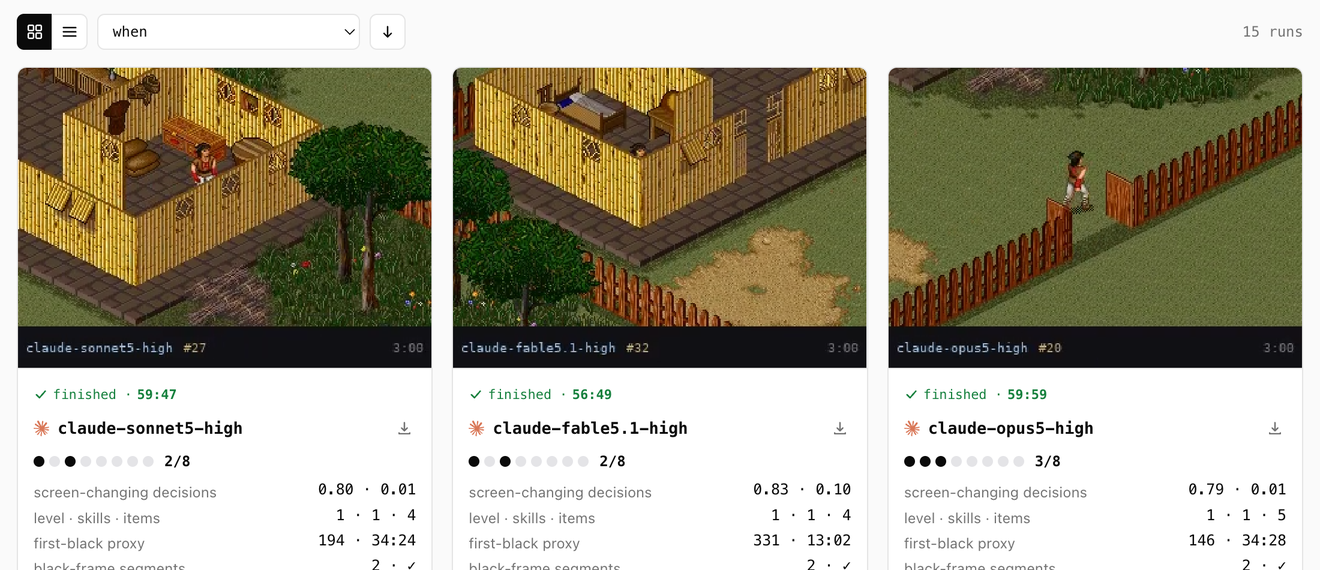
\includegraphics[height=1.14cm]{leaderboard.png}};
\node[card,fill=paperwash,minimum width=3.8cm,minimum height=2.22cm]
  (publicrun) at (4.2,-4.90) {};
\node[title] at ($(publicrun.north west)+(0.22,-0.18)$) {Public run};
\node[body] at ($(publicrun.north west)+(0.22,-0.65)$) {Replay, video\\Metrics\\Catalogue};
\path let \p1=($(boardshot.north west)-(boardshot.south west)$) in
  node[shot,anchor=north east] (replayshot) at ($(publicrun.north east)+(-0.22,-0.65)$)
  {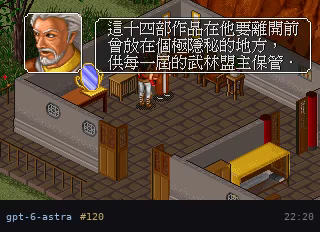
\includegraphics[height=\y1]{frames/b-hermit-talk.png}};
\draw[flow] (journal.south) -- (publicrun.north -| journal.south);
\node[vlab] at (6.13,-4.685) {render};
\draw[flow] (publicrun.west |- 0,-6.10) --
  node[lab,above=1pt] {publish} (leaderboard.east |- 0,-6.10);

% ---- Measurement: a single subsystem with two compact internal stages.
\node[card,draw=bluerule,fill=bluewash,
  minimum width=5cm,minimum height=4.07cm] (measurement) at (9,-3.05) {};
\node[title,text=blue,font=\sffamily\fontsize{8.5}{10}\selectfont\bfseries]
  at (9.25,-3.23) {Read-only measurement};
\node[note,text=blue] at (9.25,-3.63) {Not exposed by the control API};

\node[card,draw=none,minimum width=4.5cm,minimum height=1.25cm]
  (readers) at (9.25,-4.02) {};
\node[subtitle] at ($(readers.north west)+(0.2,-0.15)$) {Progress readers};
\node[small] at ($(readers.north west)+(0.2,-0.55)$)
  {Machine image: characters, bag\\Save: party, world-map position};

\node[card,draw=none,minimum width=4.5cm,minimum height=0.9cm]
  (score) at (9.25,-6.05) {};
\node[subtitle,text=blue] at ($(score.north west)+(0.2,-0.13)$) {Score};
\node[small] at ($(score.north west)+(0.2,-0.53)$)
  {Milestone ladder; completion time};

% The source arrow uses its own right-hand lane, clear of the panel header.
\draw[meas] (13.5,-2.30) -- (13.5,-4.02);
\node[vlab,text=blue] at (9.45,-2.785) {machine image; game-written save};
\draw[meas] (13.5,-5.27) -- (13.5,-6.05);
\node[vlab,text=blue] at (9.45,-5.66) {level, experience, party, books};

% Replay evidence flows into scoring; the score returns to the public run.
% Preserve replay / arrow / panels, and separate the score return below it.
\draw[meas] (8,-6.25) --
  node[mlab,above=1pt] {replay}
  node[mlab,below=1pt] {panels} (9.25,-6.25);
\draw[flow] (9.25,-6.76) -- node[lab,below=1pt] {score} (8,-6.76);
\end{tikzpicture}
\end{document}
